\scanpage{44}

globaux, comme on en voudrait. \deleted{Dernièrement} \inserted{Récemment} W.M. ont utilisé la notion de \deleted{topos} site pour définir des invariants globaux : \uline{site des relèvements de} W.M. \uline{des ouverts affines spéciaux}, pour la ``topologie de Zariski''. Sur ce site les $\Omega^\bullet_{A/k}$ forment un complexe de faisceaux, dont ils prennent l'hypercohomologie. Ils trouvent des invariants globaux intrinsèques, qui sont des modules sur $W$. Ils vérifient (?) que dans le cas envisagé au début, ils retrouvent bien $\mathbb H^*(\mathfrak X,\underline{\Omega}^\bullet_{\mathfrak X/S})$, d'où la propriété d'invariance que j'y avais énoncée.

\figure{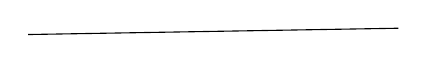
\begin{tikzpicture}\draw (0,0)--(4.7,.08);\end{tikzpicture}}

3) Critique de W.M.

C'est une idée nouvelle importante, en ce qu'elle met en relations la coh. de D.R. en car. 0, avec la cohomologie $p$-adique hypothétique, \unsure{p} Elle fournit une théorie cohomologique ``$p$-adique en car $p$'', qui échappe à une des critiques principales qu'on avait faite à D.R. naïve : elle

\margin{43}
